This part aim to control a valve for a hydraulic cylinder. Figure \ref{valve} shows the non symetric vavle driven hydraulic cylinder. 

\begin{figure}[hb]
 \includegraphics[width=\linewidth]{fig/valve.ps}
 \caption{Valve controlled hydraulic cylinder}
 \label{valve}
\end{figure}

%------------------------------------------------
% 		LEVEL 2
%------------------------------------------------
\subsection*{Level 2}
\addcontentsline{toc}{subsection}{Level 2}

We want to design a velocity controler for the valve controlled hydraulic cylinder -- using a continuous controller. 

The system will be simulate using the following reference:
\begin{itemize}
 \item $r(t) = 0.5 \text{ m/s}$
 \item Zero external force
\end{itemize}


%------------------------------------------------
% 		REAL MODEL
%------------------------------------------------
\subsubsection*{Real model}
The system is described by the following equations:

$$
\begin{array}{rcl}
    m \dot{v} & = & p_1 A_1 - p_2 A_2 - d v - f_e \\
    Q_{1v} & = & R_v \sqrt{p_s - p_1} x_v \\
    Q_{2v} & = & R_v \sqrt{p_2 - p_r} x_v \\
    Q_1 & = & Q_{1v} - Q_c \\
    Q_2 & = & - Q_{2v} + Q_c \\
    Q_c & = & A v \\
    C_f \dot{p_1} & = & Q_1 \\
    C_f \dot{p_2} & = & Q_2 \\
\end{array}
$$

With:

$p_i$: internal pression in area $i$

$m$: mass of piston

$A_i$: effective piston area

$f_e$: external force

$d$: friction coefficient

$Q_c$: volume flow due to piston velocity

$Q_{iv}$: flow from/out area $i$

$C_f$: fluid capacitance

$p_s, p_t$: supplied pression, tank pression

$R_v$: flow constant


%------------------------------------------------
% 		LINEAR MODEL
%------------------------------------------------
\subsubsection*{Linear model}
We linearize the model around an operating point:

$$\begin{array}{rcl}
   x_v & = & x_{vQ} + \Delta x_v \\
   p_1 & = & p_{1Q} + \Delta p_1 \\
   p_2 & = & p_{2Q} + \Delta p_2 \\
  \end{array}$$

Let $$x = \left[\begin{array}{ccc}x_1 & x_2 & x_3 \end{array}\right]^T = \left[\begin{array}{ccc} \Delta v & \Delta p_1 & \Delta p_2 \end{array}\right]^T$$ and $$u = \left[\begin{array}{cc}u_1 & u_2 \end{array}\right]^T = \left[\begin{array}{cc} \Delta x_v & f_e \end{array}\right]^T$$

Then:

$$ \begin{array}{rcl} 
    \bm{A} & = & \left(\frac{\partial f_i}{\partial x_j}\right)_{i,j} \\
    \bm{B} & = & \left(\frac{\partial f_i}{\partial u_j}\right)_{i,j}
   \end{array}$$
   
Thus:

$$ \begin{array}{rcl}
    \dot{x} & = &  \bm{A}x + \bm{B}u \\
    y & = & \bm{C}x + \bm{D}u
   \end{array}$$
   
With:

$$\begin{array}{rcl}
   \bm{A} & = & \left(\begin{array}{ccc} 
   -\frac{d}{m} & \frac{A}{m} & -\frac{A}{m} \\ 
   -\frac{A}{C_f} & -\frac{1}{C_f} \frac{R_v x_{vQ}}{2\sqrt{p_s - p_{1Q}}} & 0 \\ 
   \frac{A}{C_f} & 0 & \frac{1}{C_f} \frac{-R_v x_{vQ}}{2 \sqrt{p_{2Q}-p_t}}
   \end{array}\right) \\ \\
   
   \bm{B} & = & \left(\begin{array}{cc}
   0 & \frac{1}{m} \\
   \frac{R_v \sqrt{p_s - p_{1Q}}}{C_f} & 0 \\
   \frac{-R_v \sqrt{p_s - p_{1Q}}}{C_f} & 0 \\
   \end{array}\right) \\ \\
   
   \bm{C} & = & \left(\begin{array}{ccc}
   1 & 0 & 0\\
   \end{array}\right) \\ \\
   
   \bm{D} & = & 0 \\
  \end{array}$$

  
%------------------------------------------------
% 		CONTROL DESIGN
%------------------------------------------------
\subsubsection*{Control design}

% The matrix $\bm{A}$ and $\bm{B}$, using the numerical values, are:
% 
% $$\begin{array}{rcl}
%    \bm{A} & \approx & 1e9 \left(\begin{array}{ccc} 
%    0 & 0 & 0 \\ 
%    -2.86 & 0 & 0 \\ 
%    2.86 & 0 & 0
%    \end{array}\right) \\ \\
%    
%    \bm{B} & \approx & 1e11 \left(\begin{array}{cc}
%    0 & 0 \\
%    5 & 0 \\
%    5 & 0 \\
%    \end{array}\right) \\ \\
%   \end{array}$$
%   
%  \textbf{Remark:} Some values seems to be equal to zero, but are actually really small towards the other ones. Our Matlab implementation does not use zero.
 
 
 
 The close-loop transfert function is equal to:
 
 \begin{multline} 
 H(s) = \frac{B(s)}{A(s)} = \bm{C}(s\bm{I}-\bm{A})^{-1}\bm{B}
%  = \frac{1.807e7}{s^2 + 127s + 1.035e5}
 \end{multline}
  
 The system shema bloc with the controller is depicted on Figure \ref{bloc}.
 
\begin{figure}[hb]
\begin{tikzpicture}
 \sbEntree{E}
 \sbBloc{TR}{$\frac{T(s)}{R(s)}$}{E}
 \sbRelier[$r$]{E}{TR}
 \sbCompSum*{comp}{TR}{ }{ }{ }{ }
 \sbRelier{TR}{comp}
 \sbBloc{BA}{$H(s) = \frac{B(s)}{A(s)}$}{comp}
 \sbRelier[$u$]{comp}{BA}
 \sbCompSum*[5]{comp2}{BA}{ }{ }{ }{ }
 \sbSortie{S}{comp2}
 \sbRelier[$y$]{comp2}{S}
 \sbDecaleNoeudy[4]{S}{U}
 \sbCompSum*[-4]{comp3}{U}{ }{ }{ }{ }
 \sbBlocr{SR}{$\frac{S(s)}{R(s)}$}{comp3}
 \sbRelieryx{comp2-S}{comp3}
 \sbRelier{comp3}{SR}
 \sbRelierxy{SR}{comp}
 \sbDecaleNoeudy[-2]{comp2}{V}
 \sbRelier[$v$]{V}{comp2}
 \sbDecaleNoeudy[2]{comp3}{N}
 \sbRelier[$n$]{N}{comp3}
 \sbRelier{BA}{comp2}
\end{tikzpicture}
\caption{Shema bloc of the system with the controller}
\label{bloc}
\end{figure}

The control law is given by:

$$u(s) = \frac{T(s)}{R(s)} r - \frac{S(s)}{R(s)}y$$

The closed loop response is:

$$y = \frac{B}{AR+BS} r + \frac{AR}{AR+BS}v - \frac{BS}{AR+BS}n$$

Pole placement gives:

\begin{equation} AR + BS = A_m A_0 \label{poleplace} \end{equation}

We start with:

$$
\begin{array}{rcl} A_m(s) & = &  s^2 + 2 \xi_m \omega_m s + \omega_m^2 \\ A_0(s) & = & s + \omega_m' \end{array} 
$$

Therefore since:

$$\begin{array}{rcl} A(s) & =&  s^2 + 2 \xi_0 \omega_0 s + \omega_0^2 \\ B(s) & = & K_0 \end{array}$$

Equation (\ref{poleplace}) leads to:

$$\begin{array}{rcl} R(s) & =&  s+r_c \\ S(s) & = & K_C(s+s_C) \end{array}$$

We then select $T$ such as $T = A_0 t_0$.

Then:

$$\left\{\begin{array}{rcl} 
r_c & = & w_m' + 2(\omega_m \xi_m -\omega_0 \xi_0)  \\
K_C & = & \frac{1}{K_0} \left(\omega_m^2 + 2 \omega_m'^2 \xi_m \omega_m - 2 r_c \xi_0 \omega_0 - \omega_0^2\right) \\
s_C & = & \frac{1}{K_0 K_C}(\omega_m' \omega_m - r_c \omega_0^2) \\
t_0 & = & \frac{\omega_m^2}{K_0}
\end{array}\right.$$


Using the method described in the subject, we obtain the following value (satisfying step response) for $\omega_m$ and $\omega_m'$, leading to the following $A_m$ and $A_0$:

$$\begin{array}{rcl}
   A_m & = s^2 + 3600s + 4e6& \\
   A_0 & = & s+2e3\\
  \end{array}$$
  
The sensitivity function and the complementary sensitivity function are defined by:

$$\begin{array}{rcl}
   S_e(s) & = & \frac{A(s)R(s)}{A_m(s)A_0(s)} \\
   T_e(s) & = & \frac{B(s)S(s)}{A_m(s)A_0(s)}
  \end{array}$$

Figure \ref{sensitivity} show the sensitivity function and the complementary sensitivity function bode diagrams.

\begin{figure}[hb]
  \centering
  \begin{subfigure}[b]{\linewidth}
   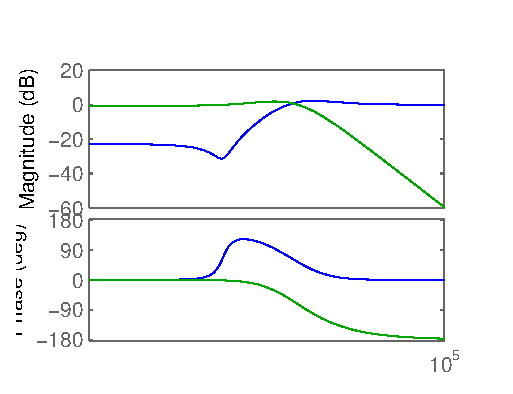
\includegraphics[width=\columnwidth]{fig/bode_SeTe_designAm.eps}
   \caption{$A_0 = s+2e3$}
  \end{subfigure}
  \begin{subfigure}[b]{\linewidth}
  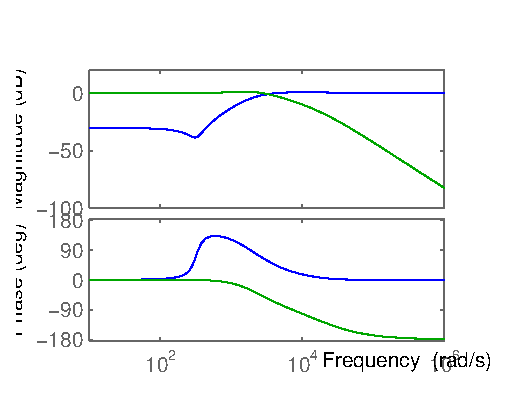
\includegraphics[width=\columnwidth]{fig/bode_SeTe_desginA0.eps}
   \caption{$A_0 = s + 2e4$}
  \end{subfigure}
 \caption{Bode diagram of the Sensitivity and complementary sensitivity functions \\ (green) -- $S_e$ \\ (blue) -- $T_e$ }
 \label{sensitivity}
\end{figure}

Figure \ref{stepIdeal} shows the step response of the system without any perturbation. 

\begin{figure}[hb]
  \centering
  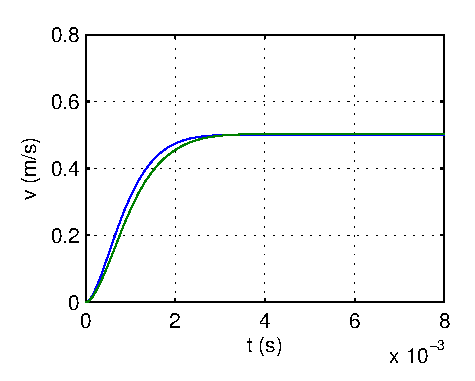
\includegraphics[width=\linewidth]{fig/step_design_Am.eps}
  \caption{Step response of the sytem without any perturbation \\ (green) -- real system \\ (blue) -- linearized system}
  \label{stepIdeal}
\end{figure}

The step response shows that:
\begin{itemize}
 \item Linearized model and real one are close to each other (the linearization was legitimate a posteriori).
 \item The system react as a second order one (as defined is the design). 
 \item The step responses present no overshoot and is fast.
 \item The non-linearized is almost as fast as the linearized one.
\end{itemize}


\clearpage

%------------------------------------------------
% 		STEP RESPONSE
%------------------------------------------------
\subsubsection*{Step response with perturbations}

Keeping the same $A_m = $, figure \ref{stepPertu} shows the step response using a perturbation $f_e = 5000\text{N}$ and the the new sensitivity function bode diagram.

\begin{figure}[hb]
  \centering
  \begin{subfigure}[b]{\linewidth}
   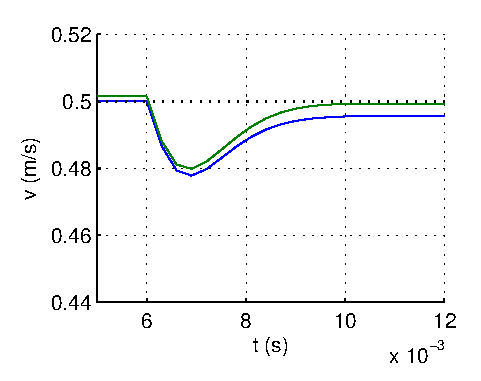
\includegraphics[width=\columnwidth]{fig/step_Fe_AmeqA0.eps}
   \caption{$A_0 = s+2e3$}
  \end{subfigure}
  \begin{subfigure}[b]{\linewidth}
  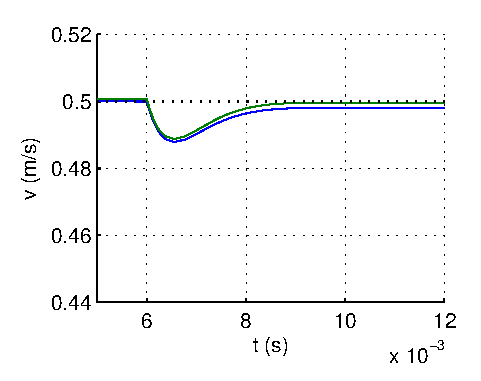
\includegraphics[width=\columnwidth]{fig/step_Fe_w0Eq10wm.eps}
   \caption{$A_0 = s + 2e4$}
  \end{subfigure}
 \caption{Step response with a perturbation $f_e = 5000 \text{N}$\\ (green) -- real system \\ (blue) -- linearized system}
 \label{stepPertu}
\end{figure}

In the first case ($A_0 = s+2e3$), the steady state error is bigger with the perturbation. This can be explain by the fact that, looking at the bode diagram, the gain is not equal to $- \infty$ with a perturbation.  
But the bigger $\omega_m'$ is, the smaller the gain is. This is why looking at the second step response, we have a smaller steady state error.

Moreover, the system is compensing the perturbation faster with a bigger $\omega_m'$ .

%------------------------------------------------
% 		MASS VARIATION
%------------------------------------------------
\subsubsection*{Mass variation}

We change the mass from $200\text{kg}$ to $100\text{kg}$. Figure \ref{mass} shows the step responses using the two same $A_0$ as in the previous subsubsection.

\begin{figure}[hb]
  \centering
  \begin{subfigure}[b]{\linewidth}
   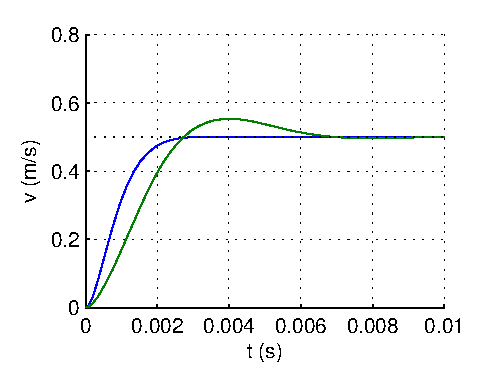
\includegraphics[width=\columnwidth]{fig/step_m_w0eqwm.eps}
   \caption{$A_0 = s+2e3$}
  \end{subfigure}
  \begin{subfigure}[b]{\linewidth}
  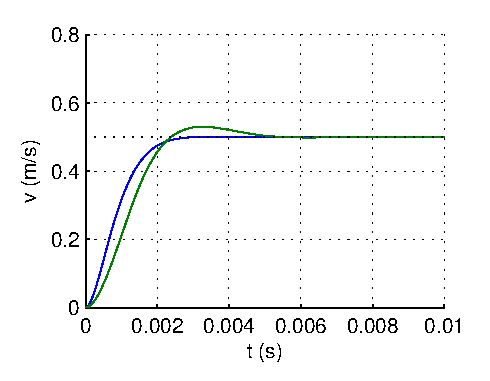
\includegraphics[width=\columnwidth]{fig/step_m_w0eq10wm.eps}
   \caption{$A_0 = s + 2e4$}
  \end{subfigure}
 \caption{Step response with a $200\text{kg}$ mass \\ (green) -- real system \\ (blue) -- linearized system}
 \label{mass}
\end{figure}

Changing the mass, the linearized system response do not change.

However, the quality of the real system response is damage by this change. Increasing the value of $\omega_m'$ leads to a better step response.

This misestimation of the parameter $m$ can be seens as the addition of noise in the model. As previously, the impact of this noise is reduce by a raise of $\omega_m'$.

%------------------------------------------------
% 		NOISE EFFECT
%------------------------------------------------
\subsubsection*{Noise effect}

In order to analyse the impact of the noise in our system, we add some noise in the feedback loop. Figure \ref{noise} shows the step response with two different $A_0$.

\begin{figure}[hb]
  \centering
  \begin{subfigure}[b]{\linewidth}
   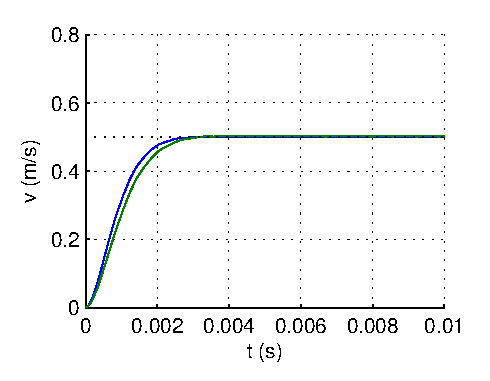
\includegraphics[width=\columnwidth]{fig/step_wm_noise.eps}
   \caption{$A_0 = s+2e3$}
  \end{subfigure}
  \begin{subfigure}[b]{\linewidth}
  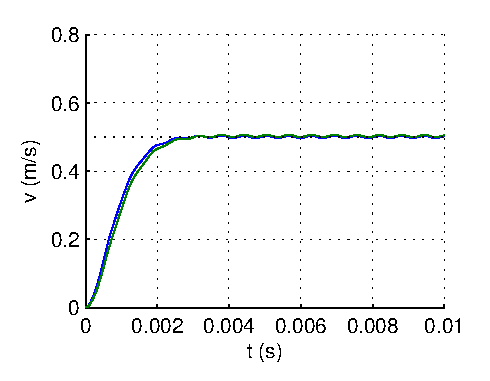
\includegraphics[width=\columnwidth]{fig/step_10wm_noise.eps}
   \caption{$A_0 = s + 2e4$}
  \end{subfigure}
 \caption{Step response with a noise \\ (green) -- real system \\ (blue) -- linearized system}
 \label{noise}
\end{figure}


The system response is worse in the second case ($\omega_m' = 2e4$). Indeed, the bode diagram shows that the cutoff frequency in this case is bigger than in the other case. The bigger $\omega_m'$, the more the noise impacts the system response.




